\chapter{Existing Environments}
\label{sec:environments}

To get an idea of how others have designed a multi agent system, we will take a look on NetLogo.\\

\section{NetLogo}
NetLogo is a widespread environment for programming a MAS. NetLogo developed by Uri Wilensky in 1999, at the Northwestern University \cite{misc:northwestern}.\\ 
\indent NetLogo features a very easy programming language for both creating agents and defining environments, NetLogo also provides a way of manipulating the cosmetics of the MAS simulation. NetLogo has the advantages that even though the programming language is simple, it is also rich on features, and can create MASes that can simulate almost any possible scenario, right from advanced traffic scenarios to how many tadpoles will survive the first week of their lives. \cite{misc:netlogolib} \\
\\
The code shown in the following code-snippet, will generate a simple test with color mixing, to simulate passing of genes.

\begin{NetLogo}{This is a NetLogo source code example.}{}
to setup
  clear-all
  ask patches
    [ set pcolor (random colors) * 10 + 5
        if pcolor = 75  ;; 75 is too close to another color so change it to 125
          [ set pcolor 125 ] ]
  reset-ticks
end

to go
  ask patches [ set pcolor [pcolor] of one-of patches ]
  tick
end


; Copyright Uri Wilensky. All rights reserved.
\end{NetLogo}

This example will, together with the NetLogo GUI, create the simulation shown in \ref{fig:NetLogoscreen}. The simulation data is saved in NetLogos custom file format, so that they can be run by someone else.

\begin{figure}[H]
\begin{center}
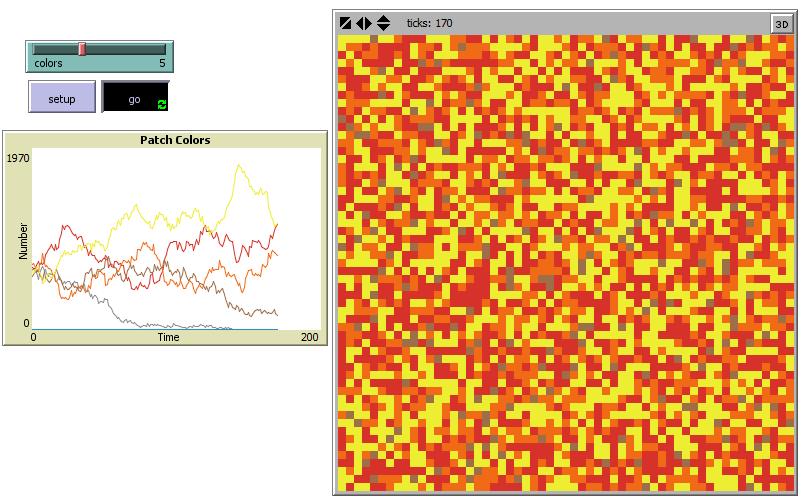
\includegraphics[scale=0.6]{Images/NetLogo.png}%
\end{center}
\caption{Simple Netlogo Simulation}%
\label{fig:NetLogoscreen}%
\end{figure}

\section{RoboCode}

Another simulation environment is RoboCode. This environment is designed to let agents (tanks) fight each other, either in teams or individually, and allows for both pre-programmed agent behavior or agents that are controlled by the user in real-time. The battlefield used by RoboCode have a user defined size and is illustrated in figure \ref{fig:RoboBattlefield}. The user of RoboCode can set up battles using pre-defined agents, or new ones can be programmed. The language is built on top of java in the form of a very extensive package. The programmer can take almost everything into account and respond to parameters with virtually any behavior he desires. Below is an example of java-code used to produce an agent usable in the RoboCode battles.

\begin{java}{The First part of a RoboCode-Robot. Note the robocode package is imported}{}
package lrn;
import robocode.*;

public class MyFirstRobot extends Robot {
\end{java}

\begin{java}{Initialization of the robot and the main loop is in the run()}{}

	public void run() {
		// Initialization of the robot should be put here

		// Robot main loop
		while(true) {
			ahead(500);
			turnLeft(50);
			turnGunRight(360);
		}
	}

\begin{java}{onScannedRobot is the method fired every time the agent sees another robot}{}

	public void onScannedRobot(ScannedRobotEvent e) {
		
		fire(1);
	}
	
\end{java}
\begin{java}{This method is run everytime the agent is hit}{}

	public void onHitByBullet(HitByBulletEvent e) {
		// Replace the next line with any behavior you would like
		back(10);
	}

\end{java}

The below code uses a method called getBearing(). This returns the heading of the object e, which in this case is the agent itself.

\begin{java}{This code describes what the agent should do when it hits a wall}{}

	public void onHitWall(HitWallEvent e) {
		back(20);
		turnLeft(e.getBearing());
		ahead(100);
	}	
}

\end{java}

\begin{figure}%
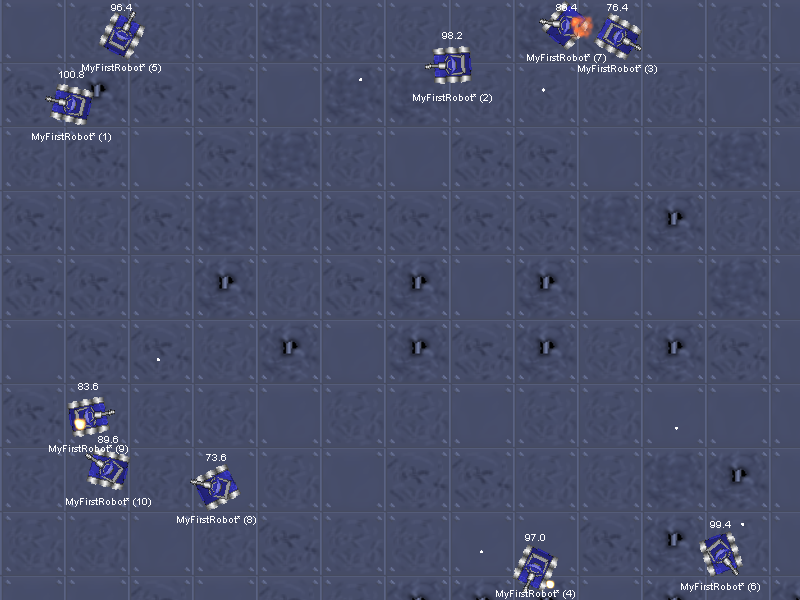
\includegraphics[width=\columnwidth]{Images/robocode_battle.png}%
\caption{The Battlefield of RoboCode}%
\label{fig:RoboBattlefield}%
\end{figure}

The language has a lot more features than described here. The whole language is described on it's webpage http://robocode.sourceforge.net.

%One example of a MAS is the NetLogo application \cite{misc:netlogo}.\\